\documentclass[1p]{elsarticle_modified}
%\bibliographystyle{elsarticle-num}

%\usepackage[colorlinks]{hyperref}
%\usepackage{abbrmath_seonhwa} %\Abb, \Ascr, \Acal ,\Abf, \Afrak
\usepackage{amsfonts}
\usepackage{amssymb}
\usepackage{amsmath}
\usepackage{amsthm}
\usepackage{scalefnt}
\usepackage{amsbsy}
\usepackage{kotex}
\usepackage{caption}
\usepackage{subfig}
\usepackage{color}
\usepackage{graphicx}
\usepackage{xcolor} %% white, black, red, green, blue, cyan, magenta, yellow
\usepackage{float}
\usepackage{setspace}
\usepackage{hyperref}

\usepackage{tikz}
\usetikzlibrary{arrows}

\usepackage{multirow}
\usepackage{array} % fixed length table
\usepackage{hhline}

%%%%%%%%%%%%%%%%%%%%%
\makeatletter
\renewcommand*\env@matrix[1][\arraystretch]{%
	\edef\arraystretch{#1}%
	\hskip -\arraycolsep
	\let\@ifnextchar\new@ifnextchar
	\array{*\c@MaxMatrixCols c}}
\makeatother %https://tex.stackexchange.com/questions/14071/how-can-i-increase-the-line-spacing-in-a-matrix
%%%%%%%%%%%%%%%

\usepackage[normalem]{ulem}

\newcommand{\msout}[1]{\ifmmode\text{\sout{\ensuremath{#1}}}\else\sout{#1}\fi}
%SOURCE: \msout is \stkout macro in https://tex.stackexchange.com/questions/20609/strikeout-in-math-mode

\newcommand{\cancel}[1]{
	\ifmmode
	{\color{red}\msout{#1}}
	\else
	{\color{red}\sout{#1}}
	\fi
}

\newcommand{\add}[1]{
	{\color{blue}\uwave{#1}}
}

\newcommand{\replace}[2]{
	\ifmmode
	{\color{red}\msout{#1}}{\color{blue}\uwave{#2}}
	\else
	{\color{red}\sout{#1}}{\color{blue}\uwave{#2}}
	\fi
}

\newcommand{\Sol}{\mathcal{S}} %segment
\newcommand{\D}{D} %diagram
\newcommand{\A}{\mathcal{A}} %arc


%%%%%%%%%%%%%%%%%%%%%%%%%%%%%5 test

\def\sl{\operatorname{\textup{SL}}(2,\Cbb)}
\def\psl{\operatorname{\textup{PSL}}(2,\Cbb)}
\def\quan{\mkern 1mu \triangleright \mkern 1mu}

\theoremstyle{definition}
\newtheorem{thm}{Theorem}[section]
\newtheorem{prop}[thm]{Proposition}
\newtheorem{lem}[thm]{Lemma}
\newtheorem{ques}[thm]{Question}
\newtheorem{cor}[thm]{Corollary}
\newtheorem{defn}[thm]{Definition}
\newtheorem{exam}[thm]{Example}
\newtheorem{rmk}[thm]{Remark}
\newtheorem{alg}[thm]{Algorithm}

\newcommand{\I}{\sqrt{-1}}
\begin{document}

%\begin{frontmatter}
%
%\title{Boundary parabolic representations of knots up to 8 crossings}
%
%%% Group authors per affiliation:
%\author{Yunhi Cho} 
%\address{Department of Mathematics, University of Seoul, Seoul, Korea}
%\ead{yhcho@uos.ac.kr}
%
%
%\author{Seonhwa Kim} %\fnref{s_kim}}
%\address{Center for Geometry and Physics, Institute for Basic Science, Pohang, 37673, Korea}
%\ead{ryeona17@ibs.re.kr}
%
%\author{Hyuk Kim}
%\address{Department of Mathematical Sciences, Seoul National University, Seoul 08826, Korea}
%\ead{hyukkim@snu.ac.kr}
%
%\author{Seokbeom Yoon}
%\address{Department of Mathematical Sciences, Seoul National University, Seoul, 08826,  Korea}
%\ead{sbyoon15@snu.ac.kr}
%
%\begin{abstract}
%We find all boundary parabolic representation of knots up to 8 crossings.
%
%\end{abstract}
%\begin{keyword}
%    \MSC[2010] 57M25 
%\end{keyword}
%
%\end{frontmatter}

%\linenumbers
%\tableofcontents
%
\newcommand\colored[1]{\textcolor{white}{\rule[-0.35ex]{0.8em}{1.4ex}}\kern-0.8em\color{red} #1}%
%\newcommand\colored[1]{\textcolor{white}{ #1}\kern-2.17ex	\textcolor{white}{ #1}\kern-1.81ex	\textcolor{white}{ #1}\kern-2.15ex\color{red}#1	}

{\Large $\underline{12a_{0491}~(K12a_{0491})}$}

\setlength{\tabcolsep}{10pt}
\renewcommand{\arraystretch}{1.6}
\vspace{1cm}\begin{tabular}{m{100pt}>{\centering\arraybackslash}m{274pt}}
\multirow{5}{120pt}{
	\centering
	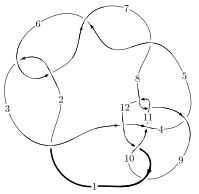
\includegraphics[width=112pt]{../../../GIT/diagram.site/Diagrams/png/1292_12a_0491.png}\\
\ \ \ A knot diagram\footnotemark}&
\allowdisplaybreaks
\textbf{Linearized knot diagam} \\
\cline{2-2}
 &
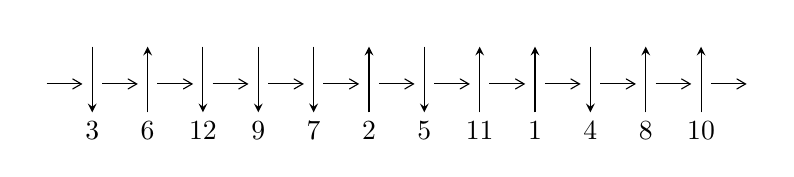
\begin{tikzpicture}[x=20pt, y=17pt]
	% nodes
	\node (C0) at (0, 0) {};
	\node (C1) at (1, 0) {};
	\node (C1U) at (1, +1) {};
	\node (C1D) at (1, -1) {3};

	\node (C2) at (2, 0) {};
	\node (C2U) at (2, +1) {};
	\node (C2D) at (2, -1) {6};

	\node (C3) at (3, 0) {};
	\node (C3U) at (3, +1) {};
	\node (C3D) at (3, -1) {12};

	\node (C4) at (4, 0) {};
	\node (C4U) at (4, +1) {};
	\node (C4D) at (4, -1) {9};

	\node (C5) at (5, 0) {};
	\node (C5U) at (5, +1) {};
	\node (C5D) at (5, -1) {7};

	\node (C6) at (6, 0) {};
	\node (C6U) at (6, +1) {};
	\node (C6D) at (6, -1) {2};

	\node (C7) at (7, 0) {};
	\node (C7U) at (7, +1) {};
	\node (C7D) at (7, -1) {5};

	\node (C8) at (8, 0) {};
	\node (C8U) at (8, +1) {};
	\node (C8D) at (8, -1) {11};

	\node (C9) at (9, 0) {};
	\node (C9U) at (9, +1) {};
	\node (C9D) at (9, -1) {1};

	\node (C10) at (10, 0) {};
	\node (C10U) at (10, +1) {};
	\node (C10D) at (10, -1) {4};

	\node (C11) at (11, 0) {};
	\node (C11U) at (11, +1) {};
	\node (C11D) at (11, -1) {8};

	\node (C12) at (12, 0) {};
	\node (C12U) at (12, +1) {};
	\node (C12D) at (12, -1) {10};
	\node (C13) at (13, 0) {};

	% arrows
	\draw[->,>={angle 60}]
	(C0) edge (C1) (C1) edge (C2) (C2) edge (C3) (C3) edge (C4) (C4) edge (C5) (C5) edge (C6) (C6) edge (C7) (C7) edge (C8) (C8) edge (C9) (C9) edge (C10) (C10) edge (C11) (C11) edge (C12) (C12) edge (C13) ;	\draw[->,>=stealth]
	(C1U) edge (C1D) (C2D) edge (C2U) (C3U) edge (C3D) (C4U) edge (C4D) (C5U) edge (C5D) (C6D) edge (C6U) (C7U) edge (C7D) (C8D) edge (C8U) (C9D) edge (C9U) (C10U) edge (C10D) (C11D) edge (C11U) (C12D) edge (C12U) ;
	\end{tikzpicture} \\
\hhline{~~} \\& 
\textbf{Solving Sequence} \\ \cline{2-2} 
 &
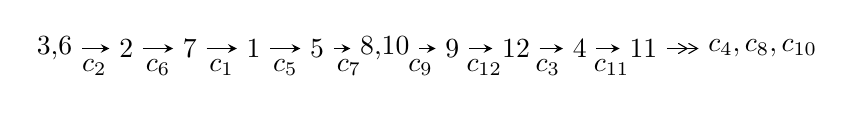
\begin{tikzpicture}[x=23pt, y=7pt]
	% node
	\node (A0) at (-1/8, 0) {3,6};
	\node (A1) at (1, 0) {2};
	\node (A2) at (2, 0) {7};
	\node (A3) at (3, 0) {1};
	\node (A4) at (4, 0) {5};
	\node (A5) at (81/16, 0) {8,10};
	\node (A6) at (49/8, 0) {9};
	\node (A7) at (57/8, 0) {12};
	\node (A8) at (65/8, 0) {4};
	\node (A9) at (73/8, 0) {11};
	\node (C1) at (1/2, -1) {$c_{2}$};
	\node (C2) at (3/2, -1) {$c_{6}$};
	\node (C3) at (5/2, -1) {$c_{1}$};
	\node (C4) at (7/2, -1) {$c_{5}$};
	\node (C5) at (9/2, -1) {$c_{7}$};
	\node (C6) at (45/8, -1) {$c_{9}$};
	\node (C7) at (53/8, -1) {$c_{12}$};
	\node (C8) at (61/8, -1) {$c_{3}$};
	\node (C9) at (69/8, -1) {$c_{11}$};
	\node (A10) at (11, 0) {$c_{4},c_{8},c_{10}$};

	% edge
	\draw[->,>=stealth]	
	(A0) edge (A1) (A1) edge (A2) (A2) edge (A3) (A3) edge (A4) (A4) edge (A5) (A5) edge (A6) (A6) edge (A7) (A7) edge (A8) (A8) edge (A9) ;
	\draw[->>,>={angle 60}]	
	(A9) edge (A10);
\end{tikzpicture} \\ 

\end{tabular} \\

\footnotetext{
The image of knot diagram is generated by the software ``\textbf{Draw programme}" developed by Andrew Bartholomew(\url{http://www.layer8.co.uk/maths/draw/index.htm\#Running-draw}), where we modified some parts for our purpose(\url{https://github.com/CATsTAILs/LinksPainter}).
}\phantom \\ \newline 
\centering \textbf{Ideals for irreducible components\footnotemark of $X_{\text{par}}$} 
 
\begin{align*}
I^u_{1}&=\langle 
36464738633053 u^{37}+59977391192807 u^{36}+\cdots+92390064679586 b+268221858684342,\\
\phantom{I^u_{1}}&\phantom{= \langle  }152917149567933 u^{37}+224240062977026 u^{36}+\cdots+184780129359172 a+822275190521781,\\
\phantom{I^u_{1}}&\phantom{= \langle  }u^{38}+2 u^{37}+\cdots+11 u+4\rangle \\
I^u_{2}&=\langle 
-264 u^{28} a+1341 u^{28}+\cdots-954 a+889,\;-4 u^{28} a-11 u^{28}+\cdots+2 a+10,\;u^{29}+u^{28}+\cdots+u-1\rangle \\
I^u_{3}&=\langle 
u^2+2 b,\;- u^2+2 a+2 u-1,\;u^4- u^3+u^2+1\rangle \\
I^u_{4}&=\langle 
2 a u+3 b+a- u+1,\;a^2+2 a-2,\;u^2+u+1\rangle \\
\\
\end{align*}
\raggedright * 4 irreducible components of $\dim_{\mathbb{C}}=0$, with total 104 representations.\\
\footnotetext{All coefficients of polynomials are rational numbers. But the coefficients are sometimes approximated in decimal forms when there is not enough margin.}
\newpage
\renewcommand{\arraystretch}{1}
\centering \section*{I. $I^u_{1}= \langle 3.65\times10^{13} u^{37}+6.00\times10^{13} u^{36}+\cdots+9.24\times10^{13} b+2.68\times10^{14},\;1.53\times10^{14} u^{37}+2.24\times10^{14} u^{36}+\cdots+1.85\times10^{14} a+8.22\times10^{14},\;u^{38}+2 u^{37}+\cdots+11 u+4 \rangle$}
\flushleft \textbf{(i) Arc colorings}\\
\begin{tabular}{m{7pt} m{180pt} m{7pt} m{180pt} }
\flushright $a_{3}=$&$\begin{pmatrix}1\\0\end{pmatrix}$ \\
\flushright $a_{6}=$&$\begin{pmatrix}0\\u\end{pmatrix}$ \\
\flushright $a_{2}=$&$\begin{pmatrix}1\\u^2\end{pmatrix}$ \\
\flushright $a_{7}=$&$\begin{pmatrix}u\\u^3+u\end{pmatrix}$ \\
\flushright $a_{1}=$&$\begin{pmatrix}u^2+1\\u^2\end{pmatrix}$ \\
\flushright $a_{5}=$&$\begin{pmatrix}u^3\\u^5+u^3+u\end{pmatrix}$ \\
\flushright $a_{8}=$&$\begin{pmatrix}u^5+u\\u^7+u^5+2 u^3+u\end{pmatrix}$ \\
\flushright $a_{10}=$&$\begin{pmatrix}-0.827563 u^{37}-1.21355 u^{36}+\cdots-4.66685 u-4.45002\\-0.394682 u^{37}-0.649176 u^{36}+\cdots-3.90259 u-2.90315\end{pmatrix}$ \\
\flushright $a_{9}=$&$\begin{pmatrix}-0.593828 u^{37}-0.803497 u^{36}+\cdots-3.09638 u-2.63169\\-0.431051 u^{37}-0.749146 u^{36}+\cdots-4.65100 u-2.78242\end{pmatrix}$ \\
\flushright $a_{12}=$&$\begin{pmatrix}-0.478729 u^{37}-0.704715 u^{36}+\cdots-1.21047 u-1.62604\\-0.261516 u^{37}-0.420727 u^{36}+\cdots-2.23130 u-2.01168\end{pmatrix}$ \\
\flushright $a_{4}=$&$\begin{pmatrix}-0.0607175 u^{37}-0.142568 u^{36}+\cdots-0.459914 u+0.0392307\\0.0514098 u^{37}+0.0422745 u^{36}+\cdots+0.976418 u+0.348449\end{pmatrix}$ \\
\flushright $a_{11}=$&$\begin{pmatrix}-0.657135 u^{37}-0.934060 u^{36}+\cdots-3.63692 u-3.16531\\-0.491481 u^{37}-0.777655 u^{36}+\cdots-4.82548 u-3.91534\end{pmatrix}$\\&\end{tabular}
\flushleft \textbf{(ii) Obstruction class $= -1$}\\~\\
\flushleft \textbf{(iii) Cusp Shapes $= \frac{140731106135951}{46195032339793} u^{37}+\frac{664007827422593}{184780129359172} u^{36}+\cdots+\frac{520000519209215}{46195032339793} u+\frac{686592782892934}{46195032339793}$}\\~\\
\newpage\renewcommand{\arraystretch}{1}
\flushleft \textbf{(iv) u-Polynomials at the component}\newline \\
\begin{tabular}{m{50pt}|m{274pt}}
Crossings & \hspace{64pt}u-Polynomials at each crossing \\
\hline $$\begin{aligned}c_{1},c_{5},c_{7}\end{aligned}$$&$\begin{aligned}
&u^{38}+10 u^{37}+\cdots+31 u+16
\end{aligned}$\\
\hline $$\begin{aligned}c_{2},c_{6}\end{aligned}$$&$\begin{aligned}
&u^{38}-2 u^{37}+\cdots-11 u+4
\end{aligned}$\\
\hline $$\begin{aligned}c_{3},c_{4}\end{aligned}$$&$\begin{aligned}
&16(16 u^{38}-24 u^{37}+\cdots+8 u+4)
\end{aligned}$\\
\hline $$\begin{aligned}c_{8},c_{9},c_{11}\\c_{12}\end{aligned}$$&$\begin{aligned}
&u^{38}-4 u^{37}+\cdots+26 u^2+1
\end{aligned}$\\
\hline $$\begin{aligned}c_{10}\end{aligned}$$&$\begin{aligned}
&u^{38}+3 u^{37}+\cdots+2944 u+512
\end{aligned}$\\
\hline
\end{tabular}\\~\\
\newpage\renewcommand{\arraystretch}{1}
\flushleft \textbf{(v) Riley Polynomials at the component}\newline \\
\begin{tabular}{m{50pt}|m{274pt}}
Crossings & \hspace{64pt}Riley Polynomials at each crossing \\
\hline $$\begin{aligned}c_{1},c_{5},c_{7}\end{aligned}$$&$\begin{aligned}
&y^{38}+38 y^{37}+\cdots-865 y+256
\end{aligned}$\\
\hline $$\begin{aligned}c_{2},c_{6}\end{aligned}$$&$\begin{aligned}
&y^{38}+10 y^{37}+\cdots+31 y+16
\end{aligned}$\\
\hline $$\begin{aligned}c_{3},c_{4}\end{aligned}$$&$\begin{aligned}
&256(256 y^{38}+1856 y^{37}+\cdots+368 y+16)
\end{aligned}$\\
\hline $$\begin{aligned}c_{8},c_{9},c_{11}\\c_{12}\end{aligned}$$&$\begin{aligned}
&y^{38}+14 y^{37}+\cdots+52 y+1
\end{aligned}$\\
\hline $$\begin{aligned}c_{10}\end{aligned}$$&$\begin{aligned}
&y^{38}-11 y^{37}+\cdots-2867200 y+262144
\end{aligned}$\\
\hline
\end{tabular}\\~\\
\newpage\flushleft \textbf{(vi) Complex Volumes and Cusp Shapes}
$$\begin{array}{c|c|c}  
\text{Solutions to }I^u_{1}& \I (\text{vol} + \sqrt{-1}CS) & \text{Cusp shape}\\
 \hline 
\begin{aligned}
u &= -0.816967 + 0.516691 I \\
a &= \phantom{-}0.66711 + 1.54872 I \\
b &= \phantom{-}0.259357 + 0.951073 I\end{aligned}
 & -2.09912 - 5.36511 I & -0.24379 + 7.67654 I \\ \hline\begin{aligned}
u &= -0.816967 - 0.516691 I \\
a &= \phantom{-}0.66711 - 1.54872 I \\
b &= \phantom{-}0.259357 - 0.951073 I\end{aligned}
 & -2.09912 + 5.36511 I & -0.24379 - 7.67654 I \\ \hline\begin{aligned}
u &= \phantom{-}0.088344 + 1.071360 I \\
a &= -0.786792 + 0.722196 I \\
b &= -0.06504 - 1.79265 I\end{aligned}
 & -8.07886 - 6.38919 I & -7.94198 + 5.19165 I \\ \hline\begin{aligned}
u &= \phantom{-}0.088344 - 1.071360 I \\
a &= -0.786792 - 0.722196 I \\
b &= -0.06504 + 1.79265 I\end{aligned}
 & -8.07886 + 6.38919 I & -7.94198 - 5.19165 I \\ \hline\begin{aligned}
u &= -0.267518 + 1.051470 I \\
a &= -1.003380 - 0.653197 I \\
b &= -0.72082 + 1.68906 I\end{aligned}
 & -2.74814 - 4.44465 I & -2.46238 + 9.81067 I \\ \hline\begin{aligned}
u &= -0.267518 - 1.051470 I \\
a &= -1.003380 + 0.653197 I \\
b &= -0.72082 - 1.68906 I\end{aligned}
 & -2.74814 + 4.44465 I & -2.46238 - 9.81067 I \\ \hline\begin{aligned}
u &= -0.430113 + 1.014270 I \\
a &= \phantom{-}1.43565 + 0.14917 I \\
b &= \phantom{-}0.515460 - 1.274350 I\end{aligned}
 & -1.89132 - 2.01335 I & \phantom{-}2.64980 + 1.56754 I \\ \hline\begin{aligned}
u &= -0.430113 - 1.014270 I \\
a &= \phantom{-}1.43565 - 0.14917 I \\
b &= \phantom{-}0.515460 + 1.274350 I\end{aligned}
 & -1.89132 + 2.01335 I & \phantom{-}2.64980 - 1.56754 I \\ \hline\begin{aligned}
u &= \phantom{-}0.414376 + 1.035890 I \\
a &= \phantom{-}1.79208 - 0.57007 I \\
b &= \phantom{-}0.67343 + 2.00434 I\end{aligned}
 & -6.1118 + 12.9461 I & -4.95394 - 9.99096 I \\ \hline\begin{aligned}
u &= \phantom{-}0.414376 - 1.035890 I \\
a &= \phantom{-}1.79208 + 0.57007 I \\
b &= \phantom{-}0.67343 - 2.00434 I\end{aligned}
 & -6.1118 - 12.9461 I & -4.95394 + 9.99096 I\\
 \hline 
 \end{array}$$\newpage$$\begin{array}{c|c|c}  
\text{Solutions to }I^u_{1}& \I (\text{vol} + \sqrt{-1}CS) & \text{Cusp shape}\\
 \hline 
\begin{aligned}
u &= \phantom{-}0.347501 + 0.797377 I \\
a &= \phantom{-}1.034560 + 0.900604 I \\
b &= \phantom{-}0.050426 - 0.214066 I\end{aligned}
 & \phantom{-}1.31226 + 1.74609 I & -8.3147 - 14.9516 I \\ \hline\begin{aligned}
u &= \phantom{-}0.347501 - 0.797377 I \\
a &= \phantom{-}1.034560 - 0.900604 I \\
b &= \phantom{-}0.050426 + 0.214066 I\end{aligned}
 & \phantom{-}1.31226 - 1.74609 I & -8.3147 + 14.9516 I \\ \hline\begin{aligned}
u &= \phantom{-}0.876268 + 0.787294 I \\
a &= \phantom{-}1.44677 - 1.98187 I \\
b &= \phantom{-}1.53330 - 1.23829 I\end{aligned}
 & \phantom{-}4.92901 - 3.34858 I & \phantom{-}2.00441 + 3.76085 I \\ \hline\begin{aligned}
u &= \phantom{-}0.876268 - 0.787294 I \\
a &= \phantom{-}1.44677 + 1.98187 I \\
b &= \phantom{-}1.53330 + 1.23829 I\end{aligned}
 & \phantom{-}4.92901 + 3.34858 I & \phantom{-}2.00441 - 3.76085 I \\ \hline\begin{aligned}
u &= \phantom{-}0.766483 + 0.236896 I \\
a &= -0.17616 + 2.12144 I \\
b &= -0.52364 + 1.60414 I\end{aligned}
 & -3.49461 - 8.73893 I & -0.20669 + 6.08042 I \\ \hline\begin{aligned}
u &= \phantom{-}0.766483 - 0.236896 I \\
a &= -0.17616 - 2.12144 I \\
b &= -0.52364 - 1.60414 I\end{aligned}
 & -3.49461 + 8.73893 I & -0.20669 - 6.08042 I \\ \hline\begin{aligned}
u &= -0.619277 + 1.044970 I \\
a &= -1.89941 + 0.04498 I \\
b &= -0.825361 + 1.032990 I\end{aligned}
 & -3.75027 + 0.04407 I & -3.65209 - 4.05484 I \\ \hline\begin{aligned}
u &= -0.619277 - 1.044970 I \\
a &= -1.89941 - 0.04498 I \\
b &= -0.825361 - 1.032990 I\end{aligned}
 & -3.75027 - 0.04407 I & -3.65209 + 4.05484 I \\ \hline\begin{aligned}
u &= -0.854926 + 0.879047 I \\
a &= -0.550203 + 0.024165 I \\
b &= \phantom{-}0.236741 + 0.729329 I\end{aligned}
 & \phantom{-}8.59748 - 1.92899 I & \phantom{-}2.35323 - 2.21681 I \\ \hline\begin{aligned}
u &= -0.854926 - 0.879047 I \\
a &= -0.550203 - 0.024165 I \\
b &= \phantom{-}0.236741 - 0.729329 I\end{aligned}
 & \phantom{-}8.59748 + 1.92899 I & \phantom{-}2.35323 + 2.21681 I\\
 \hline 
 \end{array}$$\newpage$$\begin{array}{c|c|c}  
\text{Solutions to }I^u_{1}& \I (\text{vol} + \sqrt{-1}CS) & \text{Cusp shape}\\
 \hline 
\begin{aligned}
u &= -0.912785 + 0.820153 I \\
a &= -0.94587 - 2.31254 I \\
b &= -1.27653 - 1.84714 I\end{aligned}
 & \phantom{-}2.71412 + 11.17750 I & \phantom{-}0.33746 - 5.40278 I \\ \hline\begin{aligned}
u &= -0.912785 - 0.820153 I \\
a &= -0.94587 + 2.31254 I \\
b &= -1.27653 + 1.84714 I\end{aligned}
 & \phantom{-}2.71412 - 11.17750 I & \phantom{-}0.33746 + 5.40278 I \\ \hline\begin{aligned}
u &= -0.833449 + 0.933812 I \\
a &= -0.199843 - 0.181143 I \\
b &= -0.117944 + 0.737215 I\end{aligned}
 & \phantom{-}8.42458 - 4.34753 I & \phantom{-}1.37292 + 7.42145 I \\ \hline\begin{aligned}
u &= -0.833449 - 0.933812 I \\
a &= -0.199843 + 0.181143 I \\
b &= -0.117944 - 0.737215 I\end{aligned}
 & \phantom{-}8.42458 + 4.34753 I & \phantom{-}1.37292 - 7.42145 I \\ \hline\begin{aligned}
u &= \phantom{-}0.797919 + 0.999570 I \\
a &= -2.81176 + 0.15661 I \\
b &= -1.61632 - 1.43028 I\end{aligned}
 & \phantom{-}4.26696 + 9.56924 I & \phantom{-}0.36726 - 8.73949 I \\ \hline\begin{aligned}
u &= \phantom{-}0.797919 - 0.999570 I \\
a &= -2.81176 - 0.15661 I \\
b &= -1.61632 + 1.43028 I\end{aligned}
 & \phantom{-}4.26696 - 9.56924 I & \phantom{-}0.36726 + 8.73949 I \\ \hline\begin{aligned}
u &= \phantom{-}0.885259 + 0.924982 I \\
a &= -0.402714 + 0.630130 I \\
b &= -0.426798 + 0.629711 I\end{aligned}
 & \phantom{-}7.35435 + 1.80474 I & \phantom{-}1.40236 + 2.23426 I \\ \hline\begin{aligned}
u &= \phantom{-}0.885259 - 0.924982 I \\
a &= -0.402714 - 0.630130 I \\
b &= -0.426798 - 0.629711 I\end{aligned}
 & \phantom{-}7.35435 - 1.80474 I & \phantom{-}1.40236 - 2.23426 I \\ \hline\begin{aligned}
u &= -0.349555 + 0.626590 I \\
a &= \phantom{-}0.198914 - 0.644452 I \\
b &= -0.336980 - 0.349923 I\end{aligned}
 & -0.163419 - 1.129300 I & -2.57883 + 5.23119 I \\ \hline\begin{aligned}
u &= -0.349555 - 0.626590 I \\
a &= \phantom{-}0.198914 + 0.644452 I \\
b &= -0.336980 + 0.349923 I\end{aligned}
 & -0.163419 + 1.129300 I & -2.57883 - 5.23119 I\\
 \hline 
 \end{array}$$\newpage$$\begin{array}{c|c|c}  
\text{Solutions to }I^u_{1}& \I (\text{vol} + \sqrt{-1}CS) & \text{Cusp shape}\\
 \hline 
\begin{aligned}
u &= \phantom{-}0.890869 + 0.923910 I \\
a &= \phantom{-}1.069640 + 0.049549 I \\
b &= \phantom{-}0.354749 + 0.558656 I\end{aligned}
 & \phantom{-}7.36330 + 4.74827 I & \phantom{-}1.63906 - 7.30375 I \\ \hline\begin{aligned}
u &= \phantom{-}0.890869 - 0.923910 I \\
a &= \phantom{-}1.069640 - 0.049549 I \\
b &= \phantom{-}0.354749 - 0.558656 I\end{aligned}
 & \phantom{-}7.36330 - 4.74827 I & \phantom{-}1.63906 + 7.30375 I \\ \hline\begin{aligned}
u &= -0.831961 + 0.999886 I \\
a &= \phantom{-}3.00130 - 0.50242 I \\
b &= \phantom{-}1.30372 - 1.97922 I\end{aligned}
 & \phantom{-}2.1422 - 17.6191 I & -0.56156 + 9.93310 I \\ \hline\begin{aligned}
u &= -0.831961 - 0.999886 I \\
a &= \phantom{-}3.00130 + 0.50242 I \\
b &= \phantom{-}1.30372 + 1.97922 I\end{aligned}
 & \phantom{-}2.1422 + 17.6191 I & -0.56156 - 9.93310 I \\ \hline\begin{aligned}
u &= \phantom{-}0.416803 + 0.548680 I \\
a &= -0.185246 + 1.297020 I \\
b &= \phantom{-}0.360369 - 0.039227 I\end{aligned}
 & \phantom{-}2.08077 + 1.28136 I & \phantom{-}8.26270 + 1.93719 I \\ \hline\begin{aligned}
u &= \phantom{-}0.416803 - 0.548680 I \\
a &= -0.185246 - 1.297020 I \\
b &= \phantom{-}0.360369 + 0.039227 I\end{aligned}
 & \phantom{-}2.08077 - 1.28136 I & \phantom{-}8.26270 - 1.93719 I \\ \hline\begin{aligned}
u &= -0.567270 + 0.025000 I \\
a &= \phantom{-}0.44037 - 1.76748 I \\
b &= \phantom{-}0.371874 - 0.911456 I\end{aligned}
 & \phantom{-}0.53666 - 1.46350 I & \phantom{-}5.15173 + 4.88406 I \\ \hline\begin{aligned}
u &= -0.567270 - 0.025000 I \\
a &= \phantom{-}0.44037 + 1.76748 I \\
b &= \phantom{-}0.371874 + 0.911456 I\end{aligned}
 & \phantom{-}0.53666 + 1.46350 I & \phantom{-}5.15173 - 4.88406 I\\
 \hline 
 \end{array}$$\newpage\newpage\renewcommand{\arraystretch}{1}
\centering \section*{II. $I^u_{2}= \langle -264 u^{28} a+1341 u^{28}+\cdots-954 a+889,\;-4 u^{28} a-11 u^{28}+\cdots+2 a+10,\;u^{29}+u^{28}+\cdots+u-1 \rangle$}
\flushleft \textbf{(i) Arc colorings}\\
\begin{tabular}{m{7pt} m{180pt} m{7pt} m{180pt} }
\flushright $a_{3}=$&$\begin{pmatrix}1\\0\end{pmatrix}$ \\
\flushright $a_{6}=$&$\begin{pmatrix}0\\u\end{pmatrix}$ \\
\flushright $a_{2}=$&$\begin{pmatrix}1\\u^2\end{pmatrix}$ \\
\flushright $a_{7}=$&$\begin{pmatrix}u\\u^3+u\end{pmatrix}$ \\
\flushright $a_{1}=$&$\begin{pmatrix}u^2+1\\u^2\end{pmatrix}$ \\
\flushright $a_{5}=$&$\begin{pmatrix}u^3\\u^5+u^3+u\end{pmatrix}$ \\
\flushright $a_{8}=$&$\begin{pmatrix}u^5+u\\u^7+u^5+2 u^3+u\end{pmatrix}$ \\
\flushright $a_{10}=$&$\begin{pmatrix}a\\0.228968 a u^{28}-1.16305 u^{28}+\cdots+0.827407 a-0.771032\end{pmatrix}$ \\
\flushright $a_{9}=$&$\begin{pmatrix}-0.111015 a u^{28}+0.654814 u^{28}+\cdots+0.326106 a+0.888985\\0.402428 a u^{28}-1.49870 u^{28}+\cdots+0.817866 a-0.597572\end{pmatrix}$ \\
\flushright $a_{12}=$&$\begin{pmatrix}0.990460 a u^{28}+1.17346 u^{28}+\cdots+0.715525 a-3.00954\\-0.508239 a u^{28}-1.48656 u^{28}+\cdots+0.117953 a-1.50824\end{pmatrix}$ \\
\flushright $a_{4}=$&$\begin{pmatrix}0.175195 a u^{28}-0.549003 u^{28}+\cdots+1.86036 a+11.1752\\1.55594 a u^{28}+4.61925 u^{28}+\cdots-0.695577 a+0.555941\end{pmatrix}$ \\
\flushright $a_{11}=$&$\begin{pmatrix}0.990460 a u^{28}+1.17346 u^{28}+\cdots+0.715525 a-4.00954\\-0.172593 a u^{28}-1.77103 u^{28}+\cdots-0.0555074 a-2.17259\end{pmatrix}$\\&\end{tabular}
\flushleft \textbf{(ii) Obstruction class $= -1$}\\~\\
\flushleft \textbf{(iii) Cusp Shapes $= -4 u^{28}-12 u^{26}+4 u^{25}-48 u^{24}+12 u^{23}-100 u^{22}+44 u^{21}-208 u^{20}+92 u^{19}-312 u^{18}+172 u^{17}-424 u^{16}+252 u^{15}-456 u^{14}+296 u^{13}-432 u^{12}+288 u^{11}-328 u^{10}+216 u^9-216 u^8+128 u^7-120 u^6+56 u^5-48 u^4+32 u^3-16 u^2+12 u-6$}\\~\\
\newpage\renewcommand{\arraystretch}{1}
\flushleft \textbf{(iv) u-Polynomials at the component}\newline \\
\begin{tabular}{m{50pt}|m{274pt}}
Crossings & \hspace{64pt}u-Polynomials at each crossing \\
\hline $$\begin{aligned}c_{1},c_{5},c_{7}\end{aligned}$$&$\begin{aligned}
&(u^{29}+7 u^{28}+\cdots- u-1)^{2}
\end{aligned}$\\
\hline $$\begin{aligned}c_{2},c_{6}\end{aligned}$$&$\begin{aligned}
&(u^{29}- u^{28}+\cdots+u+1)^{2}
\end{aligned}$\\
\hline $$\begin{aligned}c_{3},c_{4}\end{aligned}$$&$\begin{aligned}
&u^{58}+3 u^{57}+\cdots-2526 u+541
\end{aligned}$\\
\hline $$\begin{aligned}c_{8},c_{9},c_{11}\\c_{12}\end{aligned}$$&$\begin{aligned}
&u^{58}+9 u^{57}+\cdots+4 u+1
\end{aligned}$\\
\hline $$\begin{aligned}c_{10}\end{aligned}$$&$\begin{aligned}
&(u^{29}- u^{28}+\cdots+3 u-1)^{2}
\end{aligned}$\\
\hline
\end{tabular}\\~\\
\newpage\renewcommand{\arraystretch}{1}
\flushleft \textbf{(v) Riley Polynomials at the component}\newline \\
\begin{tabular}{m{50pt}|m{274pt}}
Crossings & \hspace{64pt}Riley Polynomials at each crossing \\
\hline $$\begin{aligned}c_{1},c_{5},c_{7}\end{aligned}$$&$\begin{aligned}
&(y^{29}+31 y^{28}+\cdots+15 y-1)^{2}
\end{aligned}$\\
\hline $$\begin{aligned}c_{2},c_{6}\end{aligned}$$&$\begin{aligned}
&(y^{29}+7 y^{28}+\cdots- y-1)^{2}
\end{aligned}$\\
\hline $$\begin{aligned}c_{3},c_{4}\end{aligned}$$&$\begin{aligned}
&y^{58}-21 y^{57}+\cdots-31273168 y+292681
\end{aligned}$\\
\hline $$\begin{aligned}c_{8},c_{9},c_{11}\\c_{12}\end{aligned}$$&$\begin{aligned}
&y^{58}+35 y^{57}+\cdots+128 y+1
\end{aligned}$\\
\hline $$\begin{aligned}c_{10}\end{aligned}$$&$\begin{aligned}
&(y^{29}-9 y^{28}+\cdots- y-1)^{2}
\end{aligned}$\\
\hline
\end{tabular}\\~\\
\newpage\flushleft \textbf{(vi) Complex Volumes and Cusp Shapes}
$$\begin{array}{c|c|c}  
\text{Solutions to }I^u_{2}& \I (\text{vol} + \sqrt{-1}CS) & \text{Cusp shape}\\
 \hline 
\begin{aligned}
u &= -0.438147 + 0.901074 I \\
a &= \phantom{-}0.866777 + 0.306748 I \\
b &= \phantom{-}0.656173 - 0.646431 I\end{aligned}
 & -1.65464 - 2.09123 I & -0.28547 + 3.54352 I \\ \hline\begin{aligned}
u &= -0.438147 + 0.901074 I \\
a &= \phantom{-}1.84101 + 0.17982 I \\
b &= \phantom{-}0.137940 - 1.357250 I\end{aligned}
 & -1.65464 - 2.09123 I & -0.28547 + 3.54352 I \\ \hline\begin{aligned}
u &= -0.438147 - 0.901074 I \\
a &= \phantom{-}0.866777 - 0.306748 I \\
b &= \phantom{-}0.656173 + 0.646431 I\end{aligned}
 & -1.65464 + 2.09123 I & -0.28547 - 3.54352 I \\ \hline\begin{aligned}
u &= -0.438147 - 0.901074 I \\
a &= \phantom{-}1.84101 - 0.17982 I \\
b &= \phantom{-}0.137940 + 1.357250 I\end{aligned}
 & -1.65464 + 2.09123 I & -0.28547 - 3.54352 I \\ \hline\begin{aligned}
u &= \phantom{-}0.409980 + 0.948974 I \\
a &= -0.583985 - 0.702562 I \\
b &= \phantom{-}0.145390 + 0.076058 I\end{aligned}
 & -2.40330 + 7.55674 I & -2.27529 - 8.69605 I \\ \hline\begin{aligned}
u &= \phantom{-}0.409980 + 0.948974 I \\
a &= -1.79153 + 0.98779 I \\
b &= -0.53216 - 1.57404 I\end{aligned}
 & -2.40330 + 7.55674 I & -2.27529 - 8.69605 I \\ \hline\begin{aligned}
u &= \phantom{-}0.409980 - 0.948974 I \\
a &= -0.583985 + 0.702562 I \\
b &= \phantom{-}0.145390 - 0.076058 I\end{aligned}
 & -2.40330 - 7.55674 I & -2.27529 + 8.69605 I \\ \hline\begin{aligned}
u &= \phantom{-}0.409980 - 0.948974 I \\
a &= -1.79153 - 0.98779 I \\
b &= -0.53216 + 1.57404 I\end{aligned}
 & -2.40330 - 7.55674 I & -2.27529 + 8.69605 I \\ \hline\begin{aligned}
u &= \phantom{-}0.273126 + 0.909412 I \\
a &= \phantom{-}1.11650 - 1.20654 I \\
b &= -0.23945 + 1.49698 I\end{aligned}
 & -7.10499 + 2.50065 I & -9.49416 - 5.21299 I \\ \hline\begin{aligned}
u &= \phantom{-}0.273126 + 0.909412 I \\
a &= -1.81954 + 1.31388 I \\
b &= -0.578605 - 0.951313 I\end{aligned}
 & -7.10499 + 2.50065 I & -9.49416 - 5.21299 I\\
 \hline 
 \end{array}$$\newpage$$\begin{array}{c|c|c}  
\text{Solutions to }I^u_{2}& \I (\text{vol} + \sqrt{-1}CS) & \text{Cusp shape}\\
 \hline 
\begin{aligned}
u &= \phantom{-}0.273126 - 0.909412 I \\
a &= \phantom{-}1.11650 + 1.20654 I \\
b &= -0.23945 - 1.49698 I\end{aligned}
 & -7.10499 - 2.50065 I & -9.49416 + 5.21299 I \\ \hline\begin{aligned}
u &= \phantom{-}0.273126 - 0.909412 I \\
a &= -1.81954 - 1.31388 I \\
b &= -0.578605 + 0.951313 I\end{aligned}
 & -7.10499 - 2.50065 I & -9.49416 + 5.21299 I \\ \hline\begin{aligned}
u &= \phantom{-}0.064282 + 0.911143 I \\
a &= -0.791876 - 0.089875 I \\
b &= \phantom{-}0.146627 + 0.566746 I\end{aligned}
 & -4.28946 - 2.39368 I & -6.11411 + 2.65936 I \\ \hline\begin{aligned}
u &= \phantom{-}0.064282 + 0.911143 I \\
a &= \phantom{-}0.79891 - 1.62494 I \\
b &= -0.167307 + 1.268310 I\end{aligned}
 & -4.28946 - 2.39368 I & -6.11411 + 2.65936 I \\ \hline\begin{aligned}
u &= \phantom{-}0.064282 - 0.911143 I \\
a &= -0.791876 + 0.089875 I \\
b &= \phantom{-}0.146627 - 0.566746 I\end{aligned}
 & -4.28946 + 2.39368 I & -6.11411 - 2.65936 I \\ \hline\begin{aligned}
u &= \phantom{-}0.064282 - 0.911143 I \\
a &= \phantom{-}0.79891 + 1.62494 I \\
b &= -0.167307 - 1.268310 I\end{aligned}
 & -4.28946 + 2.39368 I & -6.11411 - 2.65936 I \\ \hline\begin{aligned}
u &= -0.815394 + 0.851135 I \\
a &= \phantom{-}0.251672 - 1.225170 I \\
b &= -0.21594 - 1.64229 I\end{aligned}
 & -0.467923 + 0.042330 I & -2.03677 - 1.08568 I \\ \hline\begin{aligned}
u &= -0.815394 + 0.851135 I \\
a &= \phantom{-}1.94470 + 0.77465 I \\
b &= \phantom{-}0.879934 - 0.022790 I\end{aligned}
 & -0.467923 + 0.042330 I & -2.03677 - 1.08568 I \\ \hline\begin{aligned}
u &= -0.815394 - 0.851135 I \\
a &= \phantom{-}0.251672 + 1.225170 I \\
b &= -0.21594 + 1.64229 I\end{aligned}
 & -0.467923 - 0.042330 I & -2.03677 + 1.08568 I \\ \hline\begin{aligned}
u &= -0.815394 - 0.851135 I \\
a &= \phantom{-}1.94470 - 0.77465 I \\
b &= \phantom{-}0.879934 + 0.022790 I\end{aligned}
 & -0.467923 - 0.042330 I & -2.03677 + 1.08568 I\\
 \hline 
 \end{array}$$\newpage$$\begin{array}{c|c|c}  
\text{Solutions to }I^u_{2}& \I (\text{vol} + \sqrt{-1}CS) & \text{Cusp shape}\\
 \hline 
\begin{aligned}
u &= -0.886761 + 0.845005 I \\
a &= \phantom{-}0.106105 - 0.124341 I \\
b &= -0.449081 - 0.545099 I\end{aligned}
 & \phantom{-}5.93451 + 4.97924 I & \phantom{-}2.81712 - 2.83205 I \\ \hline\begin{aligned}
u &= -0.886761 + 0.845005 I \\
a &= \phantom{-}0.81426 + 1.80965 I \\
b &= \phantom{-}1.02756 + 1.59116 I\end{aligned}
 & \phantom{-}5.93451 + 4.97924 I & \phantom{-}2.81712 - 2.83205 I \\ \hline\begin{aligned}
u &= -0.886761 - 0.845005 I \\
a &= \phantom{-}0.106105 + 0.124341 I \\
b &= -0.449081 + 0.545099 I\end{aligned}
 & \phantom{-}5.93451 - 4.97924 I & \phantom{-}2.81712 + 2.83205 I \\ \hline\begin{aligned}
u &= -0.886761 - 0.845005 I \\
a &= \phantom{-}0.81426 - 1.80965 I \\
b &= \phantom{-}1.02756 - 1.59116 I\end{aligned}
 & \phantom{-}5.93451 - 4.97924 I & \phantom{-}2.81712 + 2.83205 I \\ \hline\begin{aligned}
u &= \phantom{-}0.829632 + 0.902432 I \\
a &= \phantom{-}1.44505 - 4.20042 I \\
b &= \phantom{-}2.65889 - 2.68627 I\end{aligned}
 & \phantom{-}2.66705 + 3.09358 I & \phantom{-}3.95361 - 2.70964 I \\ \hline\begin{aligned}
u &= \phantom{-}0.829632 + 0.902432 I \\
a &= -5.01880 - 0.63860 I \\
b &= -2.63453 - 2.74484 I\end{aligned}
 & \phantom{-}2.66705 + 3.09358 I & \phantom{-}3.95361 - 2.70964 I \\ \hline\begin{aligned}
u &= \phantom{-}0.829632 - 0.902432 I \\
a &= \phantom{-}1.44505 + 4.20042 I \\
b &= \phantom{-}2.65889 + 2.68627 I\end{aligned}
 & \phantom{-}2.66705 - 3.09358 I & \phantom{-}3.95361 + 2.70964 I \\ \hline\begin{aligned}
u &= \phantom{-}0.829632 - 0.902432 I \\
a &= -5.01880 + 0.63860 I \\
b &= -2.63453 + 2.74484 I\end{aligned}
 & \phantom{-}2.66705 - 3.09358 I & \phantom{-}3.95361 + 2.70964 I \\ \hline\begin{aligned}
u &= -0.796082 + 0.934420 I \\
a &= \phantom{-}1.88242 - 0.84301 I \\
b &= \phantom{-}0.15088 - 1.74671 I\end{aligned}
 & -0.72258 - 6.08103 I & -2.75508 + 6.19570 I \\ \hline\begin{aligned}
u &= -0.796082 + 0.934420 I \\
a &= -2.06357 - 0.52441 I \\
b &= -1.027530 + 0.185341 I\end{aligned}
 & -0.72258 - 6.08103 I & -2.75508 + 6.19570 I\\
 \hline 
 \end{array}$$\newpage$$\begin{array}{c|c|c}  
\text{Solutions to }I^u_{2}& \I (\text{vol} + \sqrt{-1}CS) & \text{Cusp shape}\\
 \hline 
\begin{aligned}
u &= -0.796082 - 0.934420 I \\
a &= \phantom{-}1.88242 + 0.84301 I \\
b &= \phantom{-}0.15088 + 1.74671 I\end{aligned}
 & -0.72258 + 6.08103 I & -2.75508 - 6.19570 I \\ \hline\begin{aligned}
u &= -0.796082 - 0.934420 I \\
a &= -2.06357 + 0.52441 I \\
b &= -1.027530 - 0.185341 I\end{aligned}
 & -0.72258 + 6.08103 I & -2.75508 - 6.19570 I \\ \hline\begin{aligned}
u &= \phantom{-}0.883056 + 0.860857 I \\
a &= -0.415604 + 0.501030 I \\
b &= -0.167930 + 0.016154 I\end{aligned}
 & \phantom{-}6.67034 + 1.00685 I & \phantom{-}4.05949 - 2.19242 I \\ \hline\begin{aligned}
u &= \phantom{-}0.883056 + 0.860857 I \\
a &= -0.87318 + 1.88119 I \\
b &= -1.18293 + 1.38438 I\end{aligned}
 & \phantom{-}6.67034 + 1.00685 I & \phantom{-}4.05949 - 2.19242 I \\ \hline\begin{aligned}
u &= \phantom{-}0.883056 - 0.860857 I \\
a &= -0.415604 - 0.501030 I \\
b &= -0.167930 - 0.016154 I\end{aligned}
 & \phantom{-}6.67034 - 1.00685 I & \phantom{-}4.05949 + 2.19242 I \\ \hline\begin{aligned}
u &= \phantom{-}0.883056 - 0.860857 I \\
a &= -0.87318 - 1.88119 I \\
b &= -1.18293 - 1.38438 I\end{aligned}
 & \phantom{-}6.67034 - 1.00685 I & \phantom{-}4.05949 + 2.19242 I \\ \hline\begin{aligned}
u &= -0.273342 + 0.693824 I \\
a &= -3.32819 + 2.07273 I \\
b &= \phantom{-}1.62368 + 3.27488 I\end{aligned}
 & -3.62270 - 1.16630 I & -0.21359 + 5.75923 I \\ \hline\begin{aligned}
u &= -0.273342 + 0.693824 I \\
a &= -2.49708 - 5.76954 I \\
b &= -3.05089 + 1.78246 I\end{aligned}
 & -3.62270 - 1.16630 I & -0.21359 + 5.75923 I \\ \hline\begin{aligned}
u &= -0.273342 - 0.693824 I \\
a &= -3.32819 - 2.07273 I \\
b &= \phantom{-}1.62368 - 3.27488 I\end{aligned}
 & -3.62270 + 1.16630 I & -0.21359 - 5.75923 I \\ \hline\begin{aligned}
u &= -0.273342 - 0.693824 I \\
a &= -2.49708 + 5.76954 I \\
b &= -3.05089 - 1.78246 I\end{aligned}
 & -3.62270 + 1.16630 I & -0.21359 - 5.75923 I\\
 \hline 
 \end{array}$$\newpage$$\begin{array}{c|c|c}  
\text{Solutions to }I^u_{2}& \I (\text{vol} + \sqrt{-1}CS) & \text{Cusp shape}\\
 \hline 
\begin{aligned}
u &= -0.610942 + 0.390932 I \\
a &= \phantom{-}0.147063 - 1.231320 I \\
b &= \phantom{-}0.165975 - 0.936149 I\end{aligned}
 & -0.05631 - 1.79478 I & \phantom{-}3.97960 + 2.96423 I \\ \hline\begin{aligned}
u &= -0.610942 + 0.390932 I \\
a &= -0.322053 - 1.323370 I \\
b &= -0.678870 - 0.634625 I\end{aligned}
 & -0.05631 - 1.79478 I & \phantom{-}3.97960 + 2.96423 I \\ \hline\begin{aligned}
u &= -0.610942 - 0.390932 I \\
a &= \phantom{-}0.147063 + 1.231320 I \\
b &= \phantom{-}0.165975 + 0.936149 I\end{aligned}
 & -0.05631 + 1.79478 I & \phantom{-}3.97960 - 2.96423 I \\ \hline\begin{aligned}
u &= -0.610942 - 0.390932 I \\
a &= -0.322053 + 1.323370 I \\
b &= -0.678870 + 0.634625 I\end{aligned}
 & -0.05631 + 1.79478 I & \phantom{-}3.97960 - 2.96423 I \\ \hline\begin{aligned}
u &= \phantom{-}0.840392 + 0.961339 I \\
a &= \phantom{-}0.496454 + 0.102211 I \\
b &= \phantom{-}0.314511 - 0.035083 I\end{aligned}
 & \phantom{-}6.35169 + 5.37662 I & \phantom{-}3.47961 - 2.73445 I \\ \hline\begin{aligned}
u &= \phantom{-}0.840392 + 0.961339 I \\
a &= \phantom{-}2.52374 + 0.40857 I \\
b &= \phantom{-}1.13451 + 1.54944 I\end{aligned}
 & \phantom{-}6.35169 + 5.37662 I & \phantom{-}3.47961 - 2.73445 I \\ \hline\begin{aligned}
u &= \phantom{-}0.840392 - 0.961339 I \\
a &= \phantom{-}0.496454 - 0.102211 I \\
b &= \phantom{-}0.314511 + 0.035083 I\end{aligned}
 & \phantom{-}6.35169 - 5.37662 I & \phantom{-}3.47961 + 2.73445 I \\ \hline\begin{aligned}
u &= \phantom{-}0.840392 - 0.961339 I \\
a &= \phantom{-}2.52374 - 0.40857 I \\
b &= \phantom{-}1.13451 - 1.54944 I\end{aligned}
 & \phantom{-}6.35169 - 5.37662 I & \phantom{-}3.47961 + 2.73445 I \\ \hline\begin{aligned}
u &= -0.833145 + 0.972573 I \\
a &= \phantom{-}0.422071 + 0.340573 I \\
b &= \phantom{-}0.341866 - 0.590665 I\end{aligned}
 & \phantom{-}5.53074 - 11.34930 I & \phantom{-}2.00299 + 7.67243 I \\ \hline\begin{aligned}
u &= -0.833145 + 0.972573 I \\
a &= -2.64455 + 0.38053 I \\
b &= -1.00673 + 1.69571 I\end{aligned}
 & \phantom{-}5.53074 - 11.34930 I & \phantom{-}2.00299 + 7.67243 I\\
 \hline 
 \end{array}$$\newpage$$\begin{array}{c|c|c}  
\text{Solutions to }I^u_{2}& \I (\text{vol} + \sqrt{-1}CS) & \text{Cusp shape}\\
 \hline 
\begin{aligned}
u &= -0.833145 - 0.972573 I \\
a &= \phantom{-}0.422071 - 0.340573 I \\
b &= \phantom{-}0.341866 + 0.590665 I\end{aligned}
 & \phantom{-}5.53074 + 11.34930 I & \phantom{-}2.00299 - 7.67243 I \\ \hline\begin{aligned}
u &= -0.833145 - 0.972573 I \\
a &= -2.64455 - 0.38053 I \\
b &= -1.00673 - 1.69571 I\end{aligned}
 & \phantom{-}5.53074 + 11.34930 I & \phantom{-}2.00299 - 7.67243 I \\ \hline\begin{aligned}
u &= \phantom{-}0.627727 + 0.308177 I \\
a &= \phantom{-}0.116909 - 0.679446 I \\
b &= -0.457619 - 0.120076 I\end{aligned}
 & -0.39198 - 3.74340 I & \phantom{-}3.21764 + 3.16701 I \\ \hline\begin{aligned}
u &= \phantom{-}0.627727 + 0.308177 I \\
a &= \phantom{-}0.38122 - 1.46585 I \\
b &= \phantom{-}0.541718 - 1.267480 I\end{aligned}
 & -0.39198 - 3.74340 I & \phantom{-}3.21764 + 3.16701 I \\ \hline\begin{aligned}
u &= \phantom{-}0.627727 - 0.308177 I \\
a &= \phantom{-}0.116909 + 0.679446 I \\
b &= -0.457619 + 0.120076 I\end{aligned}
 & -0.39198 + 3.74340 I & \phantom{-}3.21764 - 3.16701 I \\ \hline\begin{aligned}
u &= \phantom{-}0.627727 - 0.308177 I \\
a &= \phantom{-}0.38122 + 1.46585 I \\
b &= \phantom{-}0.541718 + 1.267480 I\end{aligned}
 & -0.39198 + 3.74340 I & \phantom{-}3.21764 - 3.16701 I \\ \hline\begin{aligned}
u &= \phantom{-}0.451236\phantom{ +0.000000I} \\
a &= \phantom{-}1.49511 + 0.78863 I \\
b &= -0.036079 + 1.103390 I\end{aligned}
 & -4.65622\phantom{ +0.000000I} & -2.67120\phantom{ +0.000000I} \\ \hline\begin{aligned}
u &= \phantom{-}0.451236\phantom{ +0.000000I} \\
a &= \phantom{-}1.49511 - 0.78863 I \\
b &= -0.036079 - 1.103390 I\end{aligned}
 & -4.65622\phantom{ +0.000000I} & -2.67120\phantom{ +0.000000I}\\
 \hline 
 \end{array}$$\newpage\newpage\renewcommand{\arraystretch}{1}
\centering \section*{III. $I^u_{3}= \langle u^2+2 b,\;- u^2+2 a+2 u-1,\;u^4- u^3+u^2+1 \rangle$}
\flushleft \textbf{(i) Arc colorings}\\
\begin{tabular}{m{7pt} m{180pt} m{7pt} m{180pt} }
\flushright $a_{3}=$&$\begin{pmatrix}1\\0\end{pmatrix}$ \\
\flushright $a_{6}=$&$\begin{pmatrix}0\\u\end{pmatrix}$ \\
\flushright $a_{2}=$&$\begin{pmatrix}1\\u^2\end{pmatrix}$ \\
\flushright $a_{7}=$&$\begin{pmatrix}u\\u^3+u\end{pmatrix}$ \\
\flushright $a_{1}=$&$\begin{pmatrix}u^2+1\\u^2\end{pmatrix}$ \\
\flushright $a_{5}=$&$\begin{pmatrix}u^3\\u^3- u^2-1\end{pmatrix}$ \\
\flushright $a_{8}=$&$\begin{pmatrix}- u^2-1\\- u^2\end{pmatrix}$ \\
\flushright $a_{10}=$&$\begin{pmatrix}\frac{1}{2} u^2- u+\frac{1}{2}\\-\frac{1}{2} u^2\end{pmatrix}$ \\
\flushright $a_{9}=$&$\begin{pmatrix}-\frac{1}{2} u^2- u-\frac{1}{2}\\-\frac{3}{2} u^2\end{pmatrix}$ \\
\flushright $a_{12}=$&$\begin{pmatrix}\frac{3}{2} u^2- u+\frac{3}{2}\\\frac{1}{2} u^2\end{pmatrix}$ \\
\flushright $a_{4}=$&$\begin{pmatrix}\frac{1}{4} u^3+\frac{1}{4}\\\frac{1}{4} u^3-\frac{1}{4} u^2-\frac{1}{4}\end{pmatrix}$ \\
\flushright $a_{11}=$&$\begin{pmatrix}\frac{1}{2} u^2- u+\frac{1}{2}\\-\frac{1}{2} u^2\end{pmatrix}$\\&\end{tabular}
\flushleft \textbf{(ii) Obstruction class $= 1$}\\~\\
\flushleft \textbf{(iii) Cusp Shapes $= -\frac{15}{4} u^3+\frac{15}{4} u^2-4 u+\frac{7}{4}$}\\~\\
\newpage\renewcommand{\arraystretch}{1}
\flushleft \textbf{(iv) u-Polynomials at the component}\newline \\
\begin{tabular}{m{50pt}|m{274pt}}
Crossings & \hspace{64pt}u-Polynomials at each crossing \\
\hline $$\begin{aligned}c_{1},c_{5}\end{aligned}$$&$\begin{aligned}
&u^4- u^3+3 u^2-2 u+1
\end{aligned}$\\
\hline $$\begin{aligned}c_{2}\end{aligned}$$&$\begin{aligned}
&u^4- u^3+u^2+1
\end{aligned}$\\
\hline $$\begin{aligned}c_{3}\end{aligned}$$&$\begin{aligned}
&16(16 u^4+8 u^3+12 u^2+4 u+1)
\end{aligned}$\\
\hline $$\begin{aligned}c_{4}\end{aligned}$$&$\begin{aligned}
&16(16 u^4-8 u^3+12 u^2-4 u+1)
\end{aligned}$\\
\hline $$\begin{aligned}c_{6}\end{aligned}$$&$\begin{aligned}
&u^4+u^3+u^2+1
\end{aligned}$\\
\hline $$\begin{aligned}c_{7}\end{aligned}$$&$\begin{aligned}
&u^4+u^3+3 u^2+2 u+1
\end{aligned}$\\
\hline $$\begin{aligned}c_{8},c_{9}\end{aligned}$$&$\begin{aligned}
&(u+1)^4
\end{aligned}$\\
\hline $$\begin{aligned}c_{10}\end{aligned}$$&$\begin{aligned}
&u^4
\end{aligned}$\\
\hline $$\begin{aligned}c_{11},c_{12}\end{aligned}$$&$\begin{aligned}
&(u-1)^4
\end{aligned}$\\
\hline
\end{tabular}\\~\\
\newpage\renewcommand{\arraystretch}{1}
\flushleft \textbf{(v) Riley Polynomials at the component}\newline \\
\begin{tabular}{m{50pt}|m{274pt}}
Crossings & \hspace{64pt}Riley Polynomials at each crossing \\
\hline $$\begin{aligned}c_{1},c_{5},c_{7}\end{aligned}$$&$\begin{aligned}
&y^4+5 y^3+7 y^2+2 y+1
\end{aligned}$\\
\hline $$\begin{aligned}c_{2},c_{6}\end{aligned}$$&$\begin{aligned}
&y^4+y^3+3 y^2+2 y+1
\end{aligned}$\\
\hline $$\begin{aligned}c_{3},c_{4}\end{aligned}$$&$\begin{aligned}
&256(256 y^4+320 y^3+112 y^2+8 y+1)
\end{aligned}$\\
\hline $$\begin{aligned}c_{8},c_{9},c_{11}\\c_{12}\end{aligned}$$&$\begin{aligned}
&(y-1)^4
\end{aligned}$\\
\hline $$\begin{aligned}c_{10}\end{aligned}$$&$\begin{aligned}
&y^4
\end{aligned}$\\
\hline
\end{tabular}\\~\\
\newpage\flushleft \textbf{(vi) Complex Volumes and Cusp Shapes}
$$\begin{array}{c|c|c}  
\text{Solutions to }I^u_{3}& \I (\text{vol} + \sqrt{-1}CS) & \text{Cusp shape}\\
 \hline 
\begin{aligned}
u &= -0.351808 + 0.720342 I \\
a &= \phantom{-}0.654246 - 0.973764 I \\
b &= \phantom{-}0.197562 + 0.253422 I\end{aligned}
 & \phantom{-}1.43393 - 1.41510 I & -0.21489 - 4.38336 I \\ \hline\begin{aligned}
u &= -0.351808 - 0.720342 I \\
a &= \phantom{-}0.654246 + 0.973764 I \\
b &= \phantom{-}0.197562 - 0.253422 I\end{aligned}
 & \phantom{-}1.43393 + 1.41510 I & -0.21489 + 4.38336 I \\ \hline\begin{aligned}
u &= \phantom{-}0.851808 + 0.911292 I \\
a &= -0.404246 - 0.135046 I \\
b &= \phantom{-}0.052438 - 0.776246 I\end{aligned}
 & \phantom{-}8.43568 + 3.16396 I & \phantom{-}3.58989 - 2.42402 I \\ \hline\begin{aligned}
u &= \phantom{-}0.851808 - 0.911292 I \\
a &= -0.404246 + 0.135046 I \\
b &= \phantom{-}0.052438 + 0.776246 I\end{aligned}
 & \phantom{-}8.43568 - 3.16396 I & \phantom{-}3.58989 + 2.42402 I\\
 \hline 
 \end{array}$$\newpage\newpage\renewcommand{\arraystretch}{1}
\centering \section*{IV. $I^u_{4}= \langle 2 a u+3 b+a- u+1,\;a^2+2 a-2,\;u^2+u+1 \rangle$}
\flushleft \textbf{(i) Arc colorings}\\
\begin{tabular}{m{7pt} m{180pt} m{7pt} m{180pt} }
\flushright $a_{3}=$&$\begin{pmatrix}1\\0\end{pmatrix}$ \\
\flushright $a_{6}=$&$\begin{pmatrix}0\\u\end{pmatrix}$ \\
\flushright $a_{2}=$&$\begin{pmatrix}1\\- u-1\end{pmatrix}$ \\
\flushright $a_{7}=$&$\begin{pmatrix}u\\u+1\end{pmatrix}$ \\
\flushright $a_{1}=$&$\begin{pmatrix}- u\\- u-1\end{pmatrix}$ \\
\flushright $a_{5}=$&$\begin{pmatrix}1\\0\end{pmatrix}$ \\
\flushright $a_{8}=$&$\begin{pmatrix}-1\\u+1\end{pmatrix}$ \\
\flushright $a_{10}=$&$\begin{pmatrix}a\\-\frac{2}{3} a u-\frac{1}{3} a+\frac{1}{3} u-\frac{1}{3}\end{pmatrix}$ \\
\flushright $a_{9}=$&$\begin{pmatrix}-\frac{1}{3} a u+\frac{1}{3} a-\frac{1}{3} u-\frac{2}{3}\\-\frac{1}{3} a u-\frac{2}{3} a+\frac{2}{3} u-\frac{2}{3}\end{pmatrix}$ \\
\flushright $a_{12}=$&$\begin{pmatrix}-\frac{2}{3} a u-\frac{1}{3} a+\frac{1}{3} u+\frac{2}{3}\\-\frac{1}{3} a u-\frac{2}{3} a-\frac{4}{3} u-\frac{2}{3}\end{pmatrix}$ \\
\flushright $a_{4}=$&$\begin{pmatrix}- a u- a+1\\\frac{2}{3} a u-\frac{2}{3} a+\frac{2}{3} u-\frac{2}{3}\end{pmatrix}$ \\
\flushright $a_{11}=$&$\begin{pmatrix}u+1\\-\frac{2}{3} a u-\frac{1}{3} a-\frac{5}{3} u-\frac{1}{3}\end{pmatrix}$\\&\end{tabular}
\flushleft \textbf{(ii) Obstruction class $= 1$}\\~\\
\flushleft \textbf{(iii) Cusp Shapes $= 4 u-4$}\\~\\
\newpage\renewcommand{\arraystretch}{1}
\flushleft \textbf{(iv) u-Polynomials at the component}\newline \\
\begin{tabular}{m{50pt}|m{274pt}}
Crossings & \hspace{64pt}u-Polynomials at each crossing \\
\hline $$\begin{aligned}c_{1},c_{5},c_{6}\end{aligned}$$&$\begin{aligned}
&(u^2- u+1)^2
\end{aligned}$\\
\hline $$\begin{aligned}c_{2},c_{7}\end{aligned}$$&$\begin{aligned}
&(u^2+u+1)^2
\end{aligned}$\\
\hline $$\begin{aligned}c_{3}\end{aligned}$$&$\begin{aligned}
&u^4-2 u^3+2 u^2-4 u+4
\end{aligned}$\\
\hline $$\begin{aligned}c_{4}\end{aligned}$$&$\begin{aligned}
&u^4+2 u^3+2 u^2+4 u+4
\end{aligned}$\\
\hline $$\begin{aligned}c_{8},c_{9},c_{11}\\c_{12}\end{aligned}$$&$\begin{aligned}
&(u^2+1)^2
\end{aligned}$\\
\hline $$\begin{aligned}c_{10}\end{aligned}$$&$\begin{aligned}
&u^4- u^2+1
\end{aligned}$\\
\hline
\end{tabular}\\~\\
\newpage\renewcommand{\arraystretch}{1}
\flushleft \textbf{(v) Riley Polynomials at the component}\newline \\
\begin{tabular}{m{50pt}|m{274pt}}
Crossings & \hspace{64pt}Riley Polynomials at each crossing \\
\hline $$\begin{aligned}c_{1},c_{2},c_{5}\\c_{6},c_{7}\end{aligned}$$&$\begin{aligned}
&(y^2+y+1)^2
\end{aligned}$\\
\hline $$\begin{aligned}c_{3},c_{4}\end{aligned}$$&$\begin{aligned}
&y^4-4 y^2+16
\end{aligned}$\\
\hline $$\begin{aligned}c_{8},c_{9},c_{11}\\c_{12}\end{aligned}$$&$\begin{aligned}
&(y+1)^4
\end{aligned}$\\
\hline $$\begin{aligned}c_{10}\end{aligned}$$&$\begin{aligned}
&(y^2- y+1)^2
\end{aligned}$\\
\hline
\end{tabular}\\~\\
\newpage\flushleft \textbf{(vi) Complex Volumes and Cusp Shapes}
$$\begin{array}{c|c|c}  
\text{Solutions to }I^u_{4}& \I (\text{vol} + \sqrt{-1}CS) & \text{Cusp shape}\\
 \hline 
\begin{aligned}
u &= -0.500000 + 0.866025 I \\
a &= \phantom{-}0.732051\phantom{ +0.000000I} \\
b &= -0.500000 - 0.133975 I\end{aligned}
 & -3.28987 - 2.02988 I & -6.00000 + 3.46410 I \\ \hline\begin{aligned}
u &= -0.500000 + 0.866025 I \\
a &= -2.73205\phantom{ +0.000000I} \\
b &= -0.50000 + 1.86603 I\end{aligned}
 & -3.28987 - 2.02988 I & -6.00000 + 3.46410 I \\ \hline\begin{aligned}
u &= -0.500000 - 0.866025 I \\
a &= \phantom{-}0.732051\phantom{ +0.000000I} \\
b &= -0.500000 + 0.133975 I\end{aligned}
 & -3.28987 + 2.02988 I & -6.00000 - 3.46410 I \\ \hline\begin{aligned}
u &= -0.500000 - 0.866025 I \\
a &= -2.73205\phantom{ +0.000000I} \\
b &= -0.50000 - 1.86603 I\end{aligned}
 & -3.28987 + 2.02988 I & -6.00000 - 3.46410 I\\
 \hline 
 \end{array}$$\newpage
\newpage\renewcommand{\arraystretch}{1}
\centering \section*{ V. u-Polynomials}
\begin{tabular}{m{50pt}|m{274pt}}
Crossings & \hspace{64pt}u-Polynomials at each crossing \\
\hline $$\begin{aligned}c_{1},c_{5}\end{aligned}$$&$\begin{aligned}
&((u^2- u+1)^2)(u^4- u^3+3 u^2-2 u+1)(u^{29}+7 u^{28}+\cdots- u-1)^{2}\\
&\cdot(u^{38}+10 u^{37}+\cdots+31 u+16)
\end{aligned}$\\
\hline $$\begin{aligned}c_{2}\end{aligned}$$&$\begin{aligned}
&((u^2+u+1)^2)(u^4- u^3+u^2+1)(u^{29}- u^{28}+\cdots+u+1)^{2}\\
&\cdot(u^{38}-2 u^{37}+\cdots-11 u+4)
\end{aligned}$\\
\hline $$\begin{aligned}c_{3}\end{aligned}$$&$\begin{aligned}
&256(u^4-2 u^3+2 u^2-4 u+4)(16 u^4+8 u^3+12 u^2+4 u+1)\\
&\cdot(16 u^{38}-24 u^{37}+\cdots+8 u+4)(u^{58}+3 u^{57}+\cdots-2526 u+541)
\end{aligned}$\\
\hline $$\begin{aligned}c_{4}\end{aligned}$$&$\begin{aligned}
&256(u^4+2 u^3+2 u^2+4 u+4)(16 u^4-8 u^3+12 u^2-4 u+1)\\
&\cdot(16 u^{38}-24 u^{37}+\cdots+8 u+4)(u^{58}+3 u^{57}+\cdots-2526 u+541)
\end{aligned}$\\
\hline $$\begin{aligned}c_{6}\end{aligned}$$&$\begin{aligned}
&((u^2- u+1)^2)(u^4+u^3+u^2+1)(u^{29}- u^{28}+\cdots+u+1)^{2}\\
&\cdot(u^{38}-2 u^{37}+\cdots-11 u+4)
\end{aligned}$\\
\hline $$\begin{aligned}c_{7}\end{aligned}$$&$\begin{aligned}
&((u^2+u+1)^2)(u^4+u^3+3 u^2+2 u+1)(u^{29}+7 u^{28}+\cdots- u-1)^{2}\\
&\cdot(u^{38}+10 u^{37}+\cdots+31 u+16)
\end{aligned}$\\
\hline $$\begin{aligned}c_{8},c_{9}\end{aligned}$$&$\begin{aligned}
&((u+1)^4)(u^2+1)^2(u^{38}-4 u^{37}+\cdots+26 u^2+1)\\
&\cdot(u^{58}+9 u^{57}+\cdots+4 u+1)
\end{aligned}$\\
\hline $$\begin{aligned}c_{10}\end{aligned}$$&$\begin{aligned}
&u^4(u^4- u^2+1)(u^{29}- u^{28}+\cdots+3 u-1)^{2}\\
&\cdot(u^{38}+3 u^{37}+\cdots+2944 u+512)
\end{aligned}$\\
\hline $$\begin{aligned}c_{11},c_{12}\end{aligned}$$&$\begin{aligned}
&((u-1)^4)(u^2+1)^2(u^{38}-4 u^{37}+\cdots+26 u^2+1)\\
&\cdot(u^{58}+9 u^{57}+\cdots+4 u+1)
\end{aligned}$\\
\hline
\end{tabular}\newpage\renewcommand{\arraystretch}{1}
\centering \section*{ VI. Riley Polynomials}
\begin{tabular}{m{50pt}|m{274pt}}
Crossings & \hspace{64pt}Riley Polynomials at each crossing \\
\hline $$\begin{aligned}c_{1},c_{5},c_{7}\end{aligned}$$&$\begin{aligned}
&((y^2+y+1)^2)(y^4+5 y^3+\cdots+2 y+1)(y^{29}+31 y^{28}+\cdots+15 y-1)^{2}\\
&\cdot(y^{38}+38 y^{37}+\cdots-865 y+256)
\end{aligned}$\\
\hline $$\begin{aligned}c_{2},c_{6}\end{aligned}$$&$\begin{aligned}
&((y^2+y+1)^2)(y^4+y^3+3 y^2+2 y+1)(y^{29}+7 y^{28}+\cdots- y-1)^{2}\\
&\cdot(y^{38}+10 y^{37}+\cdots+31 y+16)
\end{aligned}$\\
\hline $$\begin{aligned}c_{3},c_{4}\end{aligned}$$&$\begin{aligned}
&65536(y^4-4 y^2+16)(256 y^4+320 y^3+112 y^2+8 y+1)\\
&\cdot(256 y^{38}+1856 y^{37}+\cdots+368 y+16)\\
&\cdot(y^{58}-21 y^{57}+\cdots-31273168 y+292681)
\end{aligned}$\\
\hline $$\begin{aligned}c_{8},c_{9},c_{11}\\c_{12}\end{aligned}$$&$\begin{aligned}
&((y-1)^4)(y+1)^4(y^{38}+14 y^{37}+\cdots+52 y+1)\\
&\cdot(y^{58}+35 y^{57}+\cdots+128 y+1)
\end{aligned}$\\
\hline $$\begin{aligned}c_{10}\end{aligned}$$&$\begin{aligned}
&y^4(y^2- y+1)^2(y^{29}-9 y^{28}+\cdots- y-1)^{2}\\
&\cdot(y^{38}-11 y^{37}+\cdots-2867200 y+262144)
\end{aligned}$\\
\hline
\end{tabular}
\vskip 2pc
\end{document}